\documentclass{beamer}
\usepackage[utf8]{inputenc}

\usetheme{Madrid}
\usecolortheme{default}
\usepackage{amsmath,amssymb,amsfonts,amsthm}
\usepackage{txfonts}
\usepackage{tkz-euclide}
\usepackage{listings}
\usepackage{adjustbox}
\usepackage{array}
\usepackage{tabularx}
\usepackage{gvv}
\usepackage{lmodern}
\usepackage{circuitikz}
\usepackage{tikz}
\usepackage{graphicx}

\setbeamertemplate{page number in head/foot}[totalframenumber]

\usepackage{tcolorbox}
\tcbuselibrary{minted,breakable,xparse,skins}



\definecolor{bg}{gray}{0.95}
\DeclareTCBListing{mintedbox}{O{}m!O{}}{%
	breakable=true,
	listing engine=minted,
	listing only,
	minted language=#2,
	minted style=default,
	minted options={%
		linenos,
		gobble=0,
		breaklines=true,
		breakafter=,,
		fontsize=\small,
		numbersep=8pt,
		#1},
	boxsep=0pt,
	left skip=0pt,
	right skip=0pt,
	left=25pt,
	right=0pt,
	top=3pt,
	bottom=3pt,
	arc=5pt,
	leftrule=0pt,
	rightrule=0pt,
	bottomrule=2pt,
	toprule=2pt,
	colback=bg,
	colframe=orange!70,
	enhanced,
	overlay={%
		\begin{tcbclipinterior}
			\fill[orange!20!white] (frame.south west) rectangle ([xshift=20pt]frame.north west);
	\end{tcbclipinterior}},
	#3,
}
\lstset{
	language=C,
	basicstyle=\ttfamily\small,
	keywordstyle=\color{blue},
	stringstyle=\color{orange},
	commentstyle=\color{green!60!black},
	numbers=left,
	numberstyle=\tiny\color{gray},
	breaklines=true,
	showstringspaces=false,
}
%------------------------------------------------------------
%This block of code defines the information to appear in the
%Title page
\title %optional
{2.9.1}
%\subtitle{A short story}

\author % (optional)
{Hema Havil - EE25BTECH11050}



\begin{document}
	
	\frame{\titlepage}
	\begin{frame}{Question}
		Jagdish has a field which is in the shape of a right-angled triangle AQC. He wants to leave a space in the form of a square PQRS inside the field for growing wheat and the remaining space for growing vegetables. In the field, there is a pole marked as O. Based on the above information, answer the following equations\\
            (a) Taking O as the origin, P = (-200, 0) and Q = (200, 0). PQRS being a square, what are the coordinates of R and S?\\
            (b)\\  
              (i) What is the area of square PQRS ?\\
              (ii) What is the length of diagonal PR in PQRS ?\\
            (c) If S divides CA in the ratio K : 1, what is the value of K, where A = (200, 800)?
	\end{frame}

	
\begin{frame}{Theoretical Solution}
         Given that,\\ AQC is a right angled triangle at point Q and PQRS is a square inside the $\Delta$AQC,\\ 
          (a)
             We were given two points 
            \begin{align}
                P=(-200,0),Q=(200,0)
            \end{align}
            Let,\\ X be the vector along the side PQ,\\ Y be the vector along the side QR,\\Z be the vector along the side PS then, \\
            \begin{align}
                \vec{X}=\vec{Q}-\vec{P}=\myvec{200\\0}-\myvec{-200\\0}
            \end{align}
            \begin{align}
                \vec{X}=\myvec{400\\0}
            \end{align}
            
            
\end{frame}
\begin{frame}{Theoretical Solution}
        Rotation vector for 2x2 matrix is 
            \begin{align}
                \vec{R_\theta}=\myvec{cos \theta \; -sin \theta\\sin \theta\;\;\;cos \theta}
            \end{align}
            Rotate the vector $\vec{X}$ by $90^{\circ}$ anticlockwise to get Y
            \begin{align}
                \vec{Y}=\vec{R_{90}}\vec{X}
            \end{align}
            \begin{align}
                \vec{Y}=\myvec{0\;-1\\1\;\;\;\;0}\myvec{400\\0}
            \end{align}
            \begin{align}
                \vec{Y}=\myvec{0\\400}
            \end{align}
            So the vector along the side QR is $\vec{Y}=\myvec{0\\400}$ then,
            \begin{align}
                \vec{Y}=\vec{R}-\vec{Q}
            \end{align}
            
	\end{frame}
    \begin{frame}{Theoretical Solution}
        \begin{align}
                \vec{R}=\vec{Y}+\vec{Q}
            \end{align}
            \begin{align}
                \vec{R}=\myvec{0\\400}+\myvec{200\\0}
            \end{align}
            \begin{align}
                \vec{R}=\myvec{200\\400}
            \end{align}
            Since the sides QR and PS are parallel, vectors $\vec{Y}=\vec{Z}$ then
            \begin{align}
                \vec{Z}=\vec{S}-\vec{P}
            \end{align}
            \begin{align}
                \vec{S}=\vec{Z}+\vec{P}
            \end{align}
            \begin{align}
                \vec{S}=\myvec{0\\400}+\myvec{-200\\0}
            \end{align}
    \end{frame}
    \begin{frame}{Theoretical Solution}
        \begin{align}
                \vec{S}=\myvec{-200\\400}
            \end{align}
            Therefore the coordinates of the points R and S are (200,400) and (-200,400)
            (b)\\
                (i)) We know the points P(-200,0) and Q(200,0)\\
                   Let length of the side of the square PQRS be x then,
                   \begin{align}
                       x=\norm{\vec{Q}-\vec{P}}
                   \end{align}
                   \begin{align}
                       x=\norm{\myvec{400\\0}}=400
                   \end{align}\\
                Area of the square = $x^2$ = $(400)^2$ = 160000 sq units\\
                
                (ii) Length of diagnol of the square = $x\sqrt{2}$ = $400\sqrt{2}$ units\\
    \end{frame}
    \begin{frame}{Theoretical Solution}
        (c) Given the point A=(200,800)\\
            Since it was given that point S divides CA in the ratio K:1, this shows that points A,C and S are collinear. Since AQC is a right angled triangle, from this we can say that point C lies on X axis\\
            Let point C be (t,0), Consider the matrix M\\
            \begin{align}
                M = \myvec{x_1\;\;y_1\;\;1\\x_2\;\;y_2\;\;1\\x_3\;\;y_3\;\;1}
            \end{align}
            Where the points in the matrix are A(200,800),S(-200,400) and C(t,0) then,\\ substitute in equation 18
            
            
    \end{frame}
    \begin{frame}{Theoretical Solution}
           \begin{align}
                M = \myvec{200\;800\;\;1\\-200\;400\;1\\t\;\;\;\;\;0\;\;\;\;\;\;1}
            \end{align}
           {\large$R_1\rightarrow{}\frac{1}{200}R_1$}
            \begin{align}
                 M = \myvec{1\;\;\;\;\;\;4\;\;\;\;\;\frac{1}{200}\\-200\;400\;1\\t\;\;\;\;\;0\;\;\;\;\;\;1}
            \end{align}
            {\large$R_2\rightarrow{}R_2 + 200R_1$}\hspace{2cm}
            {\large$R_3\rightarrow{R_3 - tR_1}$}
            \begin{align}
                 M = \myvec{1\;\;\;\;\;\;4\;\;\;\;\;\frac{1}{200}\\0\;\;\;\;\;1200\;\;\;\;\;2\\0\;\;\;-4t\;\;\;1-\frac{t}{200}}
            \end{align}
            {\large$R_2\rightarrow{\frac{1}{200}R_2}$}
    \end{frame}
    \begin{frame}{Theoretical Solution}
            \begin{align}
                M = \myvec{1\;\;\;\;\;\;4\;\;\;\;\;\frac{1}{200}\\0\;\;\;\;\;1\;\;\;\;\;\frac{1}{600}\\0\;\;\;-4t\;\;\;1-\frac{t}{200}}
            \end{align}
            {\large$R_3\rightarrow{R_3 + 4tR_2}$}
            \begin{align}
                M = \myvec{1\;\;\;\;\;\;4\;\;\;\;\;\frac{1}{200}\\0\;\;\;\;\;1\;\;\;\;\;\frac{1}{600}\\0\;\;\;0\;\;\;\;1-\frac{t}{200}+\frac{4t}{600}}
            \end{align}
            Since the rank of matrix M is 2,
    \end{frame}
    \begin{frame}{Theoretical Solution}
        \begin{align}
                1-\frac{t}{200}+\frac{4t}{600} = 0
            \end{align}
            \begin{align}
                1 + \frac{t}{600} = 0
            \end{align}
            \begin{align}
                \frac{t}{600}=-1
            \end{align}
            \begin{align}
                t= -600
            \end{align}
            Therefore point C=(-600,0), Now S divides CA in the ratio K:1,
            \begin{align}
                S = \frac{KA+C}{K+1}
            \end{align}
    \end{frame}
    \begin{frame}{Theoretical Solution}
            \begin{align}
                K=\frac{(S-A)^T(C-S)}{\norm{S-A}^2}
            \end{align}
        \begin{align}
                K=\frac{1}{(400)^2+(400)^2}\myvec{-400\;-400}\myvec{-400\\-400}
            \end{align}
            By solving (30) we get K=1
    \end{frame}
    
	
	\begin{frame}[fragile]
	\frametitle{C Code- Ploting the given vectors}
	
	\begin{lstlisting}

#include <stdio.h>
#include <math.h>

// Output: out[0]=Rx, out[1]=Ry, out[2]=Sx, out[3]=Sy, out[4]=area, out[5]=diagonal, out[6]=Cx, out[7]=Cy, out[8]=K
void solve_from_pdf(double* out) {
    // Points from PDF
    double P[2] = {-200, 0};
    double Q[2] = {200, 0};
    double A[2] = {200, 800};

    // Side vector PQ
    double X[2] = {Q[0] - P[0], Q[1] - P[1]}; // [400, 0]
    // Rotate X by 90 deg anticlockwise to get Y (QR)
    double Y[2] = {0 - X[1], X[0]};           // [0, 400]

    // R = Q + Y = [200 + 0, 0 + 400] = [200, 400]
    
	\end{lstlisting}
\end{frame}
\begin{frame}[fragile]
\frametitle{C Code- Ploting the given vectors}
    \begin{lstlisting}
    double R[2] = {Q[0] + Y[0], Q[1] + Y[1]};

    // Z = Y, PS parallel to QR, so Z = [0, 400]
    // S = P + Z = [-200, 0 + 400] = [-200, 400]
    double S[2] = {P[0] + Y[0], P[1] + Y[1]};

    // Area and diagonal
    double x = sqrt(X[0]*X[0] + X[1]*X[1]);   // 400
    double area = x * x;
    double diag = x * sqrt(2);

    // Point C from PDF, lying on x-axis, with collinearity
    double C[2] = {-600, 0}; // from matrix rank/collinearity in PDF
    \end{lstlisting}
\end{frame}
\begin{frame}[fragile]
   \frametitle{C Code- Ploting the given vectors}
    \begin{lstlisting}
        // K for S dividing CA in K:1
    // S = (K*A + C)/(K+1) --> solve for K using x or y (use y)
    double K = (S[1] - C[1]) / (A[1] - S[1]);

    out[0] = R[0];
    out[1] = R[1];
    out[2] = S[0];
    out[3] = S[1];
    out[4] = area;
    out[5] = diag;
    out[6] = C[0];
    out[7] = C[1];
    out[8] = K;
}
    \end{lstlisting}
\end{frame}

\begin{frame}[fragile]
	\frametitle{Python Code using shared output}
	\begin{lstlisting}
		import ctypes
import numpy as np
import matplotlib.pyplot as plt

# Load the compiled shared C lib (use correct path if needed)
lib = ctypes.CDLL('./2.9.1.so')

# Set up output variables
outputs = (ctypes.c_double * 9)()
lib.solve_from_pdf(outputs)

# Extract variables (variable names as in C and PDF)
R = (outputs[0], outputs[1])
S = (outputs[2], outputs[3])
area = outputs[4]
diagonal = outputs[5]
C = (outputs[6], outputs[7])
K = outputs[8]



	\end{lstlisting}
\end{frame}
\begin{frame}[fragile]
	\frametitle{Python Code using shared output}
	\begin{lstlisting}	
    P = (-200, 0)
Q = (200, 0)
A = (200, 800)
O = (0, 0)

# --- Print for verification ---
print("Coordinates of R:", R)
print("Coordinates of S:", S)
print("Area of PQRS:", area)
print("Length of diagonal PR:", diagonal)
print("Coordinates of C:", C)
print("Value of K:", K)

# --- Plot as in the PDF ---
plt.figure(figsize=(9,9))
# Triangle AQC (A,Q,C)
triangle_x = [A[0], Q[0], C[0], A[0]]
triangle_y = [A[1], Q[1], C[1], A[1]]

	\end{lstlisting}
\end{frame}
\begin{frame}[fragile]
	\frametitle{Python Code using shared output}
	\begin{lstlisting}
plt.plot(triangle_x, triangle_y, 'k-', label='Triangle AQC', linewidth=2)

# Square PQRS
square_x = [P[0], Q[0], R[0], S[0], P[0]]
square_y = [P[1], Q[1], R[1], S[1], P[1]]
plt.plot(square_x, square_y, 'b-', label='Square PQRS', linewidth=2)

plt.scatter([O[0], P[0], Q[0], A[0], R[0], S[0], C[0]],
            [O[1], P[1], Q[1], A[1], R[1], S[1], C[1]], color='red')
for pt, name in zip([O, P, Q, A, R, S, C], ['O', 'P', 'Q', 'A', 'R', 'S', 'C']):
    plt.text(pt[0]+10, pt[1]+20, name, fontsize=13)

# Diagonal PR in square
plt.plot([P[0], R[0]], [P[1], R[1]], 'r--', label='Diagonal PR')


	\end{lstlisting}
\end{frame}
\begin{frame}[fragile]
        \frametitle{Python Code using shared output}
      \begin{lstlisting}
          # Annotate area & diagonal
plt.text(-350, 200, f'Area = {area:.0f}', fontsize=13, color='blue', bbox=dict(facecolor='white', alpha=0.7))
plt.text(-350, 120, f'Diagonal = {diagonal:.1f}', fontsize=13, color='purple', bbox=dict(facecolor='white', alpha=0.7))

plt.xlabel('x')
plt.ylabel('y')
plt.xlim(-700, 300)
plt.ylim(-100, 900)
plt.grid(True)
plt.legend()
plt.title('Triangle AQC & Square PQRS (as per PDF solution)')
plt.tight_layout()
plt.show()
      \end{lstlisting}
\end{frame}
\begin{frame}{Plot by python using shared output}
	\begin{center}
	\begin{figure}[H]
		\centering
		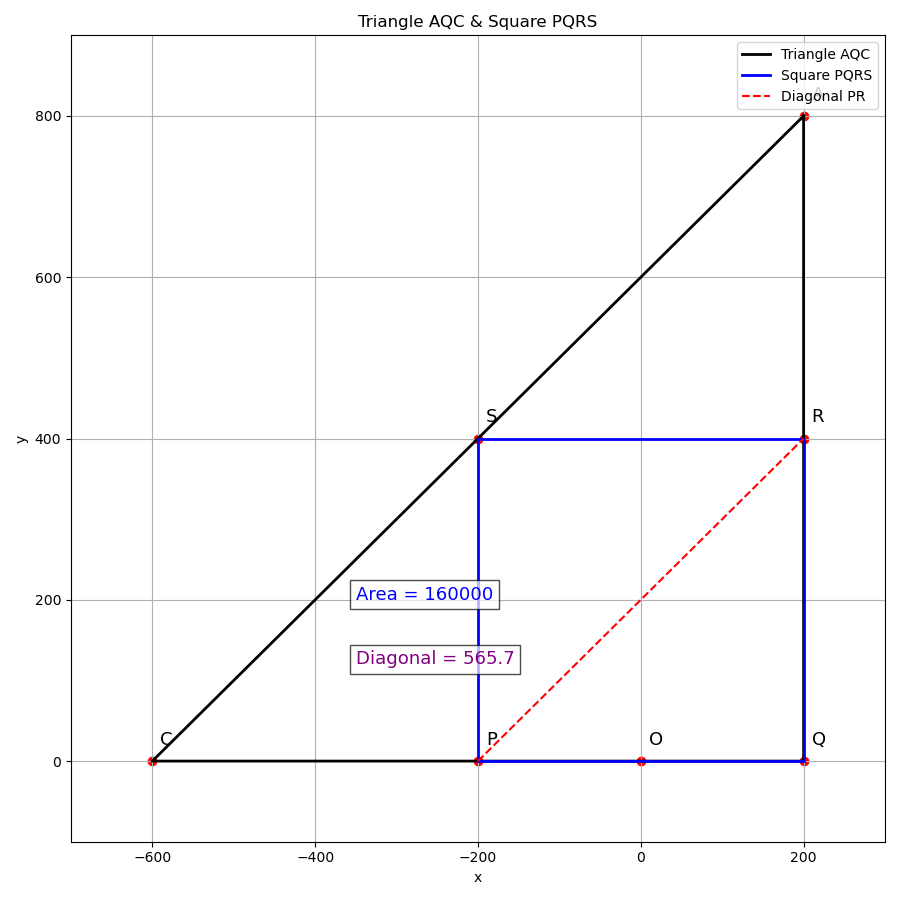
\includegraphics[width = 0.7\columnwidth]{figs/fig1.png}
		\caption{Plot of the vectors when y=3}
		\label{fig1}
	\end{figure}
	\end{center}
\end{frame}
\begin{frame}[fragile]
     \frametitle{Python code for the plot}
\begin{lstlisting}
   import numpy as np
import matplotlib.pyplot as plt

# Given points (from solution and problem statement)
P = np.array([-200, 0])
Q = np.array([200, 0])
A = np.array([200, 800])
O = np.array([0, 0])

# Step 1: Vector from P to Q
X = Q - P  # [400, 0]

# Step 2: Rotate X by 90 degrees anticlockwise to get Y (QR)
Y = np.array([0 - X[1], X[0]])  # [0, 400]

# Step 3: Find R and S using vector addition as in PDF
R = Q + Y     # [200, 400]
S = P + Y     # [-200, 400]


\end{lstlisting}
\end{frame}
\begin{frame}[fragile]
   \frametitle{Python code for the plot}
    \begin{lstlisting}
# Lists for square
square_x = [P[0], Q[0], R[0], S[0], P[0]]
square_y = [P[1], Q[1], R[1], S[1], P[1]]

plt.figure(figsize=(8, 8))

# Plot triangle
plt.plot(triangle_x, triangle_y, 'r-', label='Triangle')

# Plot square
plt.plot(square_x, square_y, 'b-', label='Square')

# Label triangle points
plt.text(A[0], A[1], 'A')
plt.text(Q[0], Q[1], 'Q')
plt.text(C[0], C[1], 'C')



 \end{lstlisting}
\end{frame}
 \begin{frame}[fragile]
       \frametitle{Python code for the plot}
       \begin{lstlisting}
      # Step 4: Area and diagonal of the square
side = np.linalg.norm(X)         # 400
area = side ** 2                 # 160000
diagonal = side * np.sqrt(2)     # 400*sqrt(2) ≈ 565.69

# Step 5: Find C as in PDF by solving with collinearity (x-axis, so y=0)
# Using determinant as in PDF: |A-Q| |C-Q| = 0 for being collinear with Q as origin
# But given in PDF as C = (-600, 0)
C = np.array([-600, 0])

# Step 6: Find K for S dividing CA in K:1, S = (K*A + C)/(K+1)
# Solve for K using y-coordinates
S_y = S[1]
K = (S_y - C[1]) / (A[1] - S_y)


    \end{lstlisting}
 \end{frame}
 \begin{frame}[fragile]
     \frametitle{Python code for the plot}
     \begin{lstlisting}
         # ---- Plot as in the PDF ----
plt.figure(figsize=(9,9))
# Triangle AQC (A->Q->C->A)
triangle_x = [A[0], Q[0], C[0], A[0]]
triangle_y = [A[1], Q[1], C[1], A[1]]
plt.plot(triangle_x, triangle_y, 'k-', label='Triangle AQC', linewidth=2)

# Square PQRS
square_x = [P[0], Q[0], R[0], S[0], P[0]]
square_y = [P[1], Q[1], R[1], S[1], P[1]]
plt.plot(square_x, square_y, 'b-', label='Square PQRS', linewidth=2)

# Points O, P, Q, A, R, S, C
pts = [O, P, Q, A, R, S, C]
lbls = ['O', 'P', 'Q', 'A', 'R', 'S', 'C']
for pt, name in zip(pts, lbls):
    

     \end{lstlisting}
 \end{frame}
 \begin{frame}[fragile]
   \frametitle{Python code for the plot}
     \begin{lstlisting}
         plt.scatter(pt[0], pt[1], color='red')
    plt.text(pt[0]+10, pt[1]+20, name, fontsize=13)

# Diagonal PR
plt.plot([P[0], R[0]], [P[1], R[1]], 'r--', label='Diagonal PR')

# Area, Diagonal annotations
plt.text(-350, 200, f'Area = {area:.0f}', fontsize=13, color='blue', bbox=dict(facecolor='white', alpha=0.7))
plt.text(-350, 120, f'Diagonal = {diagonal:.2f}', fontsize=13, color='purple', bbox=dict(facecolor='white', alpha=0.7))

plt.xlabel('x')
plt.ylabel('y')
plt.xlim(-700, 300)
plt.ylim(-100, 900)
plt.grid(True)

     \end{lstlisting}
 \end{frame}
 \begin{frame}[fragile]
      \frametitle{Python code for the plot}
     \begin{lstlisting}
         plt.legend()
plt.title('Triangle AQC & Square PQRS (PDF method, pure Python)')
plt.tight_layout()
plt.show()

# For verification
print("Coordinates of R:", tuple(R))
print("Coordinates of S:", tuple(S))
print("Area of PQRS:", area)
print("Length of diagonal PR:", diagonal)
print("Coordinates of C:", tuple(C))
print("Value of K:", K)
     \end{lstlisting}
 \end{frame}
     \begin{frame}{Plot of triangle and square}
       \begin{figure}
           \centering
           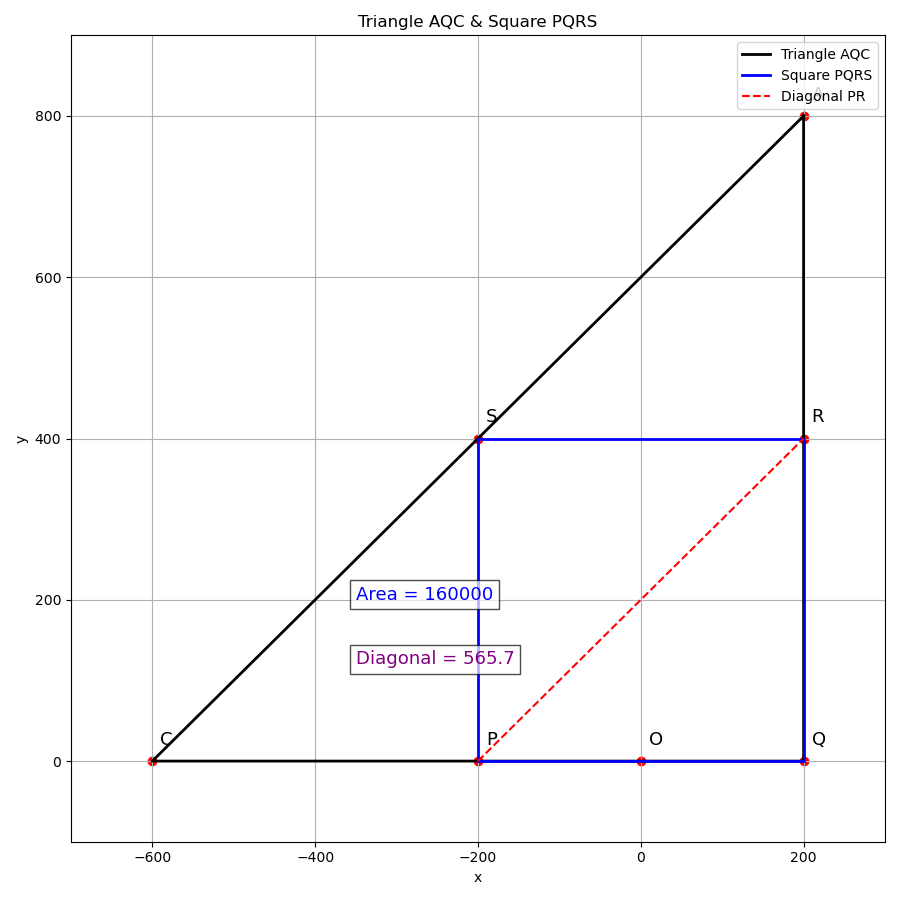
\includegraphics[width=0.7\linewidth]{figs/fig1.png}
           \caption{Plot of the points}
           \label{fig:placeholder}
       \end{figure}
         
     \end{frame}
\end{document}
